\chapter{Galáxias peculiares aneladas}

As galáxias aneladas, RGs (ring galaxies) ou ``galáxias em anel'', possuem a aparência de um anel, e a origem de sua estrutura mais discutida é que são frutos de acidentes cósmicos de proporções gigantescas \cite{Appleton96}. Uma das primeiras galáxias aneladas apresentadas foi a \emph{Cartwheel}\footnote{Identificação de outros catálogos: AM 0035-335, ESO 350-40 e HRG 35002.}, Figura~\ref{fig:cartwheel}, localizada na constelação do Escultor, descoberta pelo astrônomo suíço Fritz Zwicky, em 1941. As RGs, geralmente, têm seu núcleo localizado em uma posição assimétrica em relação ao anel e podem possuir estruturas como nódulos nos anéis, i. e. regiões que têm alta taxa de formação estelar, filamentos, deformações e assimetrias \cite{2016lago}. 

O astrônomo americano Halton Arp publicou em 1966 o \emph{Atlas of peculiar galaxies} \cite{1966Arp} que contém 338 imagens de galáxias do hemisfério norte, agrupadas de forma a reunir objetos com estruturas exóticas e semelhantes. A classificação das galáxias aneladas foi feita pela primeira vez por \citeonline{1976ApJ...208..650T}, com base no catálogo de Arp (1966), denominando-as por R (do inglês \emph{ring}). Em 1987, \emph{A catalogue of southern peculiar galaxies and associations} \cite{1987arpmadore} categorizou 489 galáxias peculiares do hemisfério sul, em 25 tipos morfológicos, sendo a sexta categoria, as RGs. O estudo desses objetos pode nos auxiliar a compreender alguns dos processos de perturbações e interações mais surpreendentes entre as galáxias, e também, nos confrontar com outros que não compreendemos.

Os anéis, comumente azuis comparados a outras galáxias normais, possuem condensações de regiões HII, onde há atividade de formação estelar intensa, ideia suportada por observações espectrográficas por \citeonline{2011fogarty}. Estudos mais precisos dos anéis, e casos particulares, são necessários para certificar que constituem de fato toda a galáxia e que realmente têm forma de anel no espaço, e não conchas esféricas ou um efeito de absorção de matéria peculiarmente distribuída \cite{Agosto1970}, para desta forma obter uma caracterização de propriedades das RG e classificar qualitativamente suas morfologias peculiares de acordo com classes e sub-classes. Pesquisas com dados fotométricos mostram que os anéis possuem formação estelar intensa, e em algumas RGs, o anel é o único lugar onde estas novas estrelas estão se formando. Estes anéis, ou melhor, experimentos de perturbação em escala galáctica, podem ser usados para ilustrar os efeitos da força potencial gravitacional da galáxia alvo, bem como mecanismos que levam ao nascimento e morte de estrelas na propagação de ondas de densidade \cite{Appleton96}, ferramentas atraentes para a compreensão da estrutura e evolução galáctica, mesmo que colisão entre duas galáxias seja um evento raro.

\begin{figure}
  \centering 
  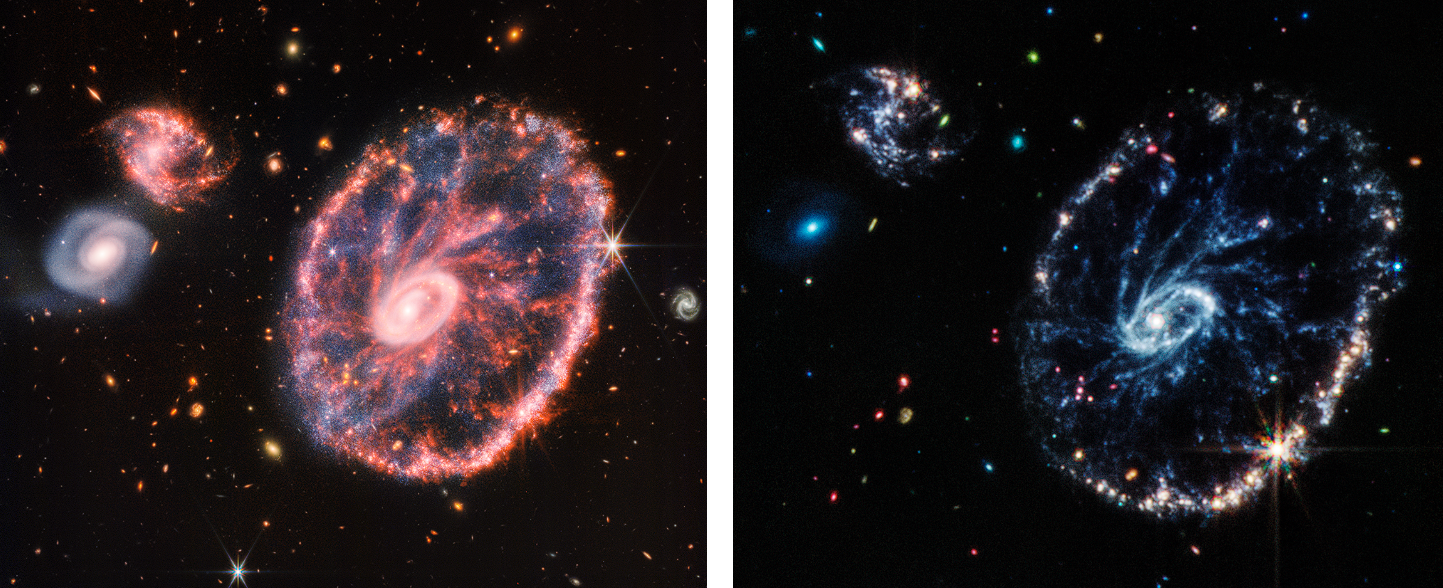
\includegraphics[width=0.8\textwidth]{Imagens/Cartwheel03.PNG} 
  \caption[Gálaxia Cartwheel.]{Esquerda: imagem no infravermelho próximo (NIRCam) e infravermelho médio (MIRI), detalhando os brilhantes anéis, interno e externo, da Grande Cartwheel. Direita: imagem no infravermelho médio (MIRI) onde se observa grande taxa de formação estelar no anel externo, enquanto que na região central há maior concentração de poeira e aglomerados de estrelas. Imagens capturadas pelo Telescópio Espacial James Webb. Créditos: NASA, ESA, CSA, STSci. O astrônomo Zwicky ao observar Cartwheel com uma câmera Schmidt de 18 polegadas na montanha Palomar em 1941, disse que esta galáxia representava "uma das estruturas mais complicadas que aguardam explicação com base na dinâmica estelar".}
  \label{fig:cartwheel} 
\end{figure}


\section{Morfologia peculiar}

A morfologia peculiar das RGs pode ser classificada por dois processos físicos: quando os anéis são fruto de interações com o meio ou com outras galáxias, denomina-se como peculiares (peculiar ring galaxy - PRG) e estes objetos são bem raros, aproximadamente um a cada $10^\text{4}$ \cite{1987bin}; ou quando a origem do anel se deve a ressonância da barra de uma galáxia espiral ou perturbações do fluxo de gás do interior da galáxia, são classificados como ressonantes (normal ring galaxy - NRG), observado em galáxias SB(r), Sa(r) e SAB \cite{1998abans, 1995Buta}. Na maioria dos casos de NRG, o anel interno possui mesma idade, composição química e cor da galáxia. Anteriormente, por  \citeonline{1986Madore}, também foi proposta esta classificação, tipo-O para as RGs com anéis ressonantes, e para os anéis clássicos colisionais, tipo-P. Os anéis foram classificados por três tipos de fenômenos físicos distintos por \citeonline{1995Buta}: normal ou de ressonância, que se forma por ação de torques gravitacionais; de colisão, se origina por uma onda de choque expansiva do gás através da colisão com uma galáxia companheira; e polar, onde o anel consiste em um disco inclinado ao plano de uma galáxia, sendo fruto de uma fusão disruptiva. Atualmente, a melhor classificação morfológica das classes e subclasses das RGs é a de \citeonline{1998abans}, que categorizaram visualmente 489 PRGs do catálogo “Catalogue of Southern
Peculiar Galaxies and Associations” de Arp \& Madore, e dividiram os anéis em cinco categorias, ilustradas na Tabela~\ref{tab:minha_tabela} e Figura~\ref{fig:quadro}: 

\begin{table}[h]
  \centering
  \begin{tabular}{ccc}
    \toprule
    \textbf{Famílias de Anéis} & \textbf{Código} & \textbf{Estruturas básicas} \\
    \midrule
    Polar & P & (a) Spindle; (b) Saturn; (c) Worm-like \\
    Hoag & H & (a) Hoag; (b) Hoag-like \\
    Elíptico & E & (a) Nódulos; (b) Suave; (c) Solitário \\
    Irregular & I &  \\
    Centralmente Suave & CS &  \\
    \bottomrule
  \end{tabular}
  \caption{Classificação dos anéis\protect\footnotemark.}
  \label{tab:minha_tabela}
\end{table}
\footnotetext{Tabela adaptada de \cite{1998abans}.}

Esta divisão de classes e subclasses está relacionada com as características e mecanismos de formação dos anéis, de acordo com o tamanho e formato, elipticidade e presença de um bojo no interior do anel ou nele próprio. A estrutura dos anéis do tipo Polar são resultado da acreção ou fusão de matéria rica em gás de uma companheira próxima. À estas RGs da família Polar, são atribuídas três estruturas básicas: Spindle (fuso ou eixo alongado), que possui anel em forma de fuso e perpendicular (ou quase) ao eixo da galáxia; Saturn (Saturno), galáxia com núcleo (bojo) esférico ou elíptico e anel redondo; Worm-like (tipo minhoca), contém um bojo alongado semelhante a uma minhoca e anel com um nódulo (região de forte formação estelar) \cite{1998abans}. Os objetos da família Hoag, o nome vem de Arthur Hoag, astrônomo americano que descobriu em 1950 uma RG nomeada posteriormente de objeto de Hoag (galáxia PGC 54559), possuem um notável anel circular ao redor do bojo e são divididos em dois tipos: Hoag, os anéis possuem simetria circular e um bojo difuso; Hoag-like (semelhante ao Hoag), possui anel e bojo característicos de baixa elipticidade ou bojo esférico grande comparado ao Hoag. Os anéis classificados como elípticos, são mais alongados como o formato de uma elipse e subdivididos em: com nódulos, regiões de intensa formação estelar e o bojo se encontra um pouco deslocado do centro do anel; suave, o gás que constitui o anel se distribui de forma suave em torno do bojo; e solitário, quando o núcleo (bojo) da galáxia se encontra no anel (anel com um único nódulo). As RGs categorizadas com anéis irregulares, possuem o formato pseudo-anéis ou anéis vazios com nódulos, sem um bojo localizado na região central do anel ou deslocado, e à família dos anéis centralmente suaves, são galáxias em forma anelada com nódulos e de aparência difusa, em que não se encontra uma protuberância ou bojo definidos. Exemplos das classes de NRG e PRG são ilustradas na Figura~\ref{fig:quadro}.

O estudo das galáxias aneladas peculiares, que representam, em todos os casos, interações passadas ou em andamento \cite{1983AJ}, traz informações importantes dos processos interativos em escala galáctica que ocorrem no Universo, permite a observação do berçário de estrelas nos anéis, a dinâmica e trilhas evolutivas estelares.

\begin{figure}
  \centering 
  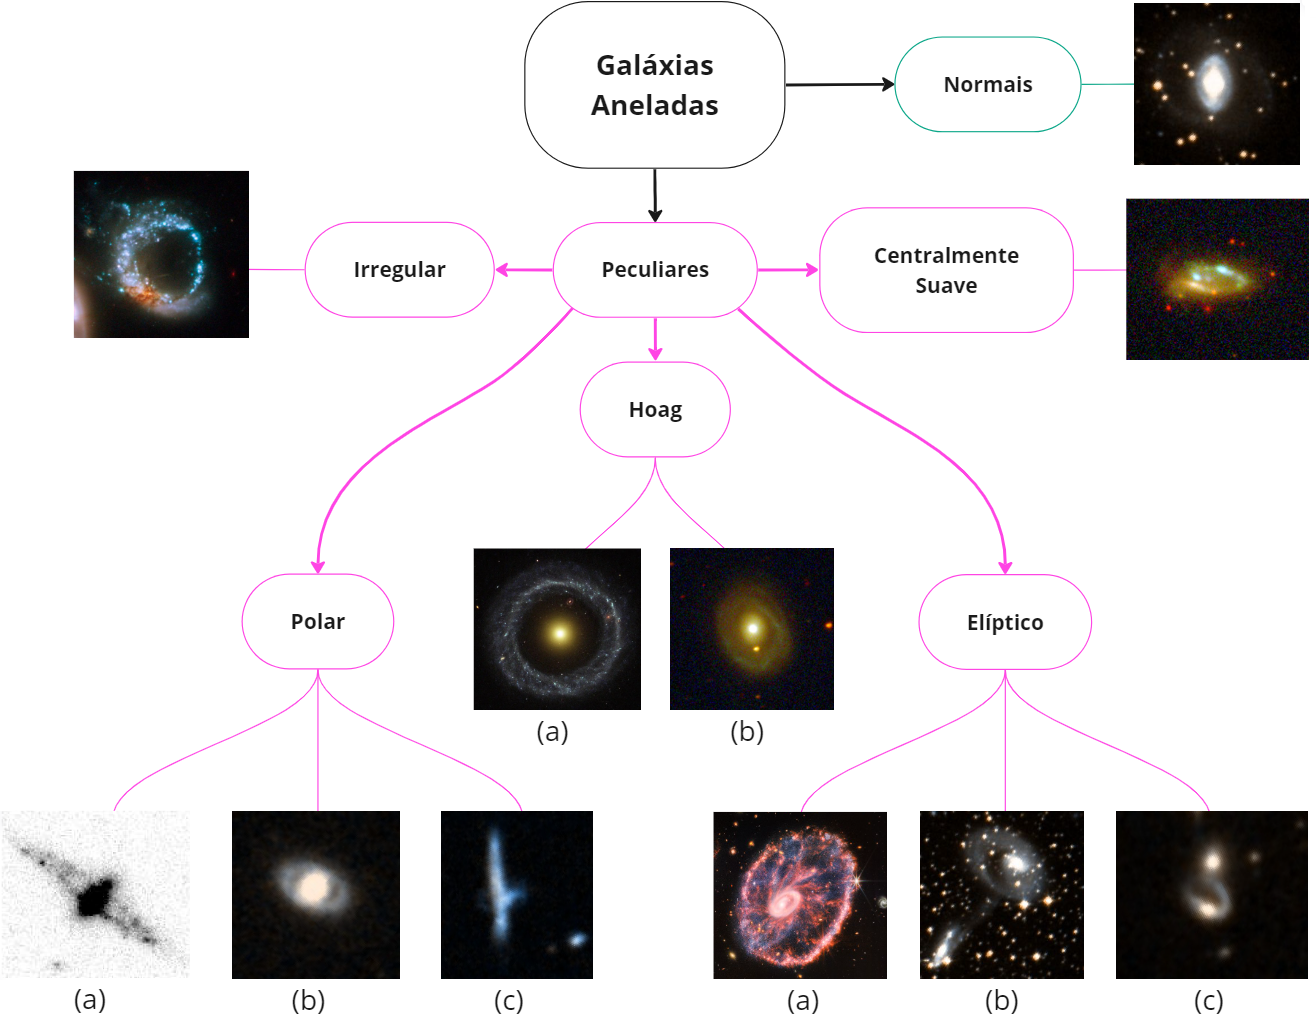
\includegraphics[width=1.0\textwidth]{Imagens/quadro.png} 
  \caption[Família dos anéis]{Polar (a) Spindle: A0136 0801, créditos: \cite{1995AIPC}; Polar (b) Saturn: HRG 54103, Polar (c) Worm-like: ESO 199-IG12, Elíptico (b) Suave: HRG 13801, Elíptico (c) Solitário: ESO 189-2, créditos: Digitized Sky Survey, STScI/NASA e CDS; Centralmente Suave: HRG 50201, Hoag (b) Hoag-like: AM 0425-421, créditos: S-PLUS; Elíptico (a) Nódulos: HRG 35002, crédito: NASA, ESA, CSA e STScI; Hoag (a): PGC 54559, crédito: NASA, R. Lucas e STScI/AURA; Irregular: ARP 147, créditos: NASA's Hubble Space Telescope. Diagrama adaptado pela classificação de \citeonline{1998abans} e construído pela autora.}
  \label{fig:quadro} 
\end{figure}


\section{Estudo dos processos interativos}

Em 1950 quando o astrônomo Hoag estudava o objeto PGC 54559, achava que provavelmente seria uma nebulosa planetária ou um fenômeno de lente gravitacional (anel de Einstein), porque na época não tinham imagens ou observações detalhadas suficientes para calcular a distância do anel e do núcleo (bojo) para afirmar que estavam à mesma distância e que portanto, seriam tudo o mesmo objeto. Em 1987, \citeonline{1987sch} confirmaram que tanto o anel circular brilhante quanto o núcleo de PGC 54559 estavam à mesma distância e que constituíam uma galáxia como um todo, apresentando observações fotométricas e espectroscópicas. Na década de 70, Theys e Spiegel realizaram um estudo de propriedades observacionais básicas sobre a estrutura de um conjunto de RGs, onde sugerem que, em sua maioria, o anel se forma devido a uma perturbação gravitacional na galáxia hospedeira, possibilitando o estudo da dinâmica galáctica entre os objetos interagentes. Contribuição seguinte feita por Lynds e Toomre, com as primeiras simulações computacionais numéricas de interações galácticas, para entender a formação dos anéis.

\begin{figure}[h]
  \centering 
  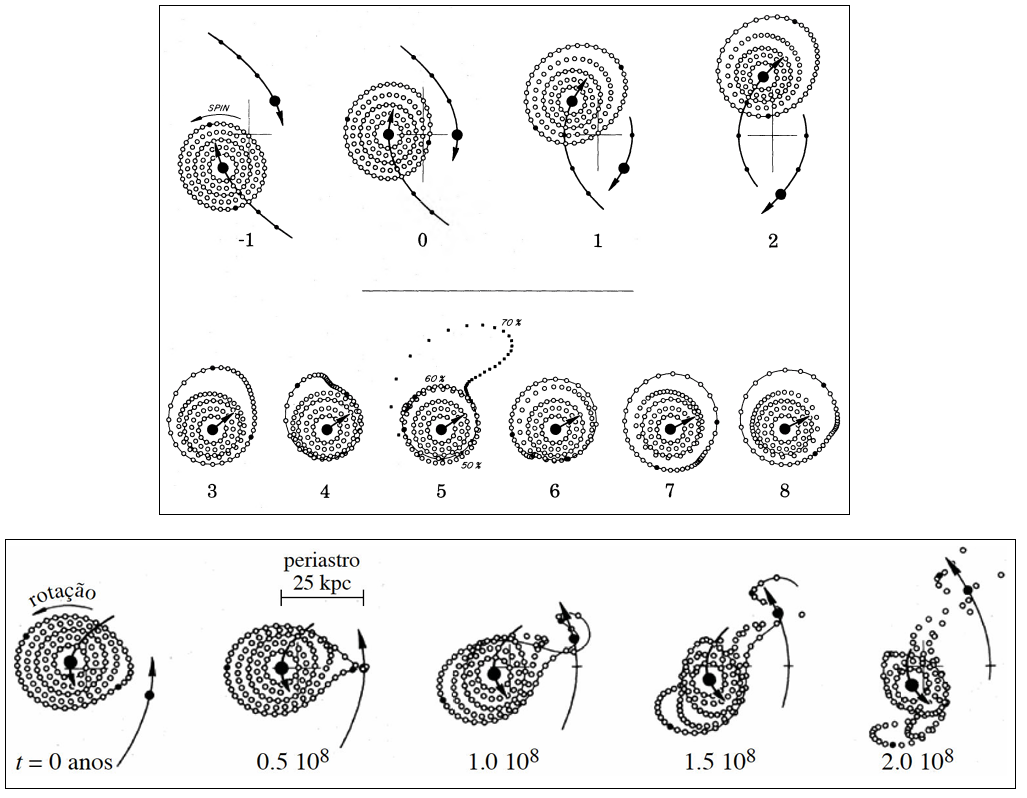
\includegraphics[width=0.8\textwidth]{Imagens/tmtmsimu.png} 
  \caption[Simulação de partículas teste.]{Acima: Simulação da passagem parabólica retrógrada de um objeto companheiro de mesma massa, onde se observa a interpenetrações parciais dos anéis mais externos e suas oscilações. Abaixo: Simulação da passagem próxima de uma galáxia anã de uma espiral. Créditos: \cite{1972ApJ...178..623T}}
  \label{fig:simulacaotmtm} 
\end{figure}

\begin{figure}[h]
  \centering 
  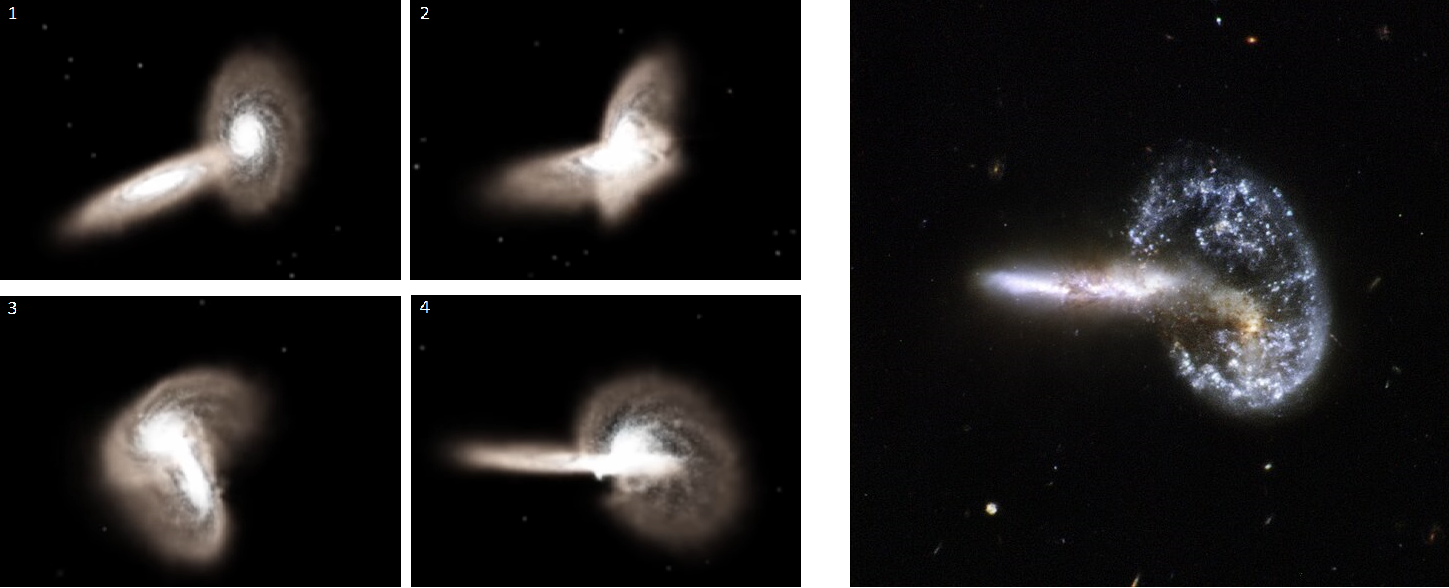
\includegraphics[width=0.8\textwidth]{Imagens/simuvsobs.png} 
  \caption[Simulação vs. Observação.]{Esquerda: simulação da interação entre duas galáxias espirais, crédito: Summers, 2008. Direita: ARP 148, crédito: NASA, ESA, the Hubble Heritage (STScI/AURA) e A. Evans (University of Virginia, Charlottesville/NRAO/Stony Brook University).}
  \label{fig:simulacao} 
\end{figure}

Quando se compara as classes de galáxias aneladas peculiares Polar e Hoag, por exemplo, há uma diferença de posição do anel em relação ao núcleo da galáxia. Nas galáxias polares pode-se ver claramente em suas formas a fusão de galáxias e a força gravitacional entre elas causada pela interação, apresentando uma estrutura de anel catastrófico e o gás ``espalhado'' entorno da galáxia. Os objetos Hoag, por outro lado, são perfeitamente estruturados como se tivessem sido formados por um processo calmo e perfeito.

\begin{figure}[h]
  \centering 
  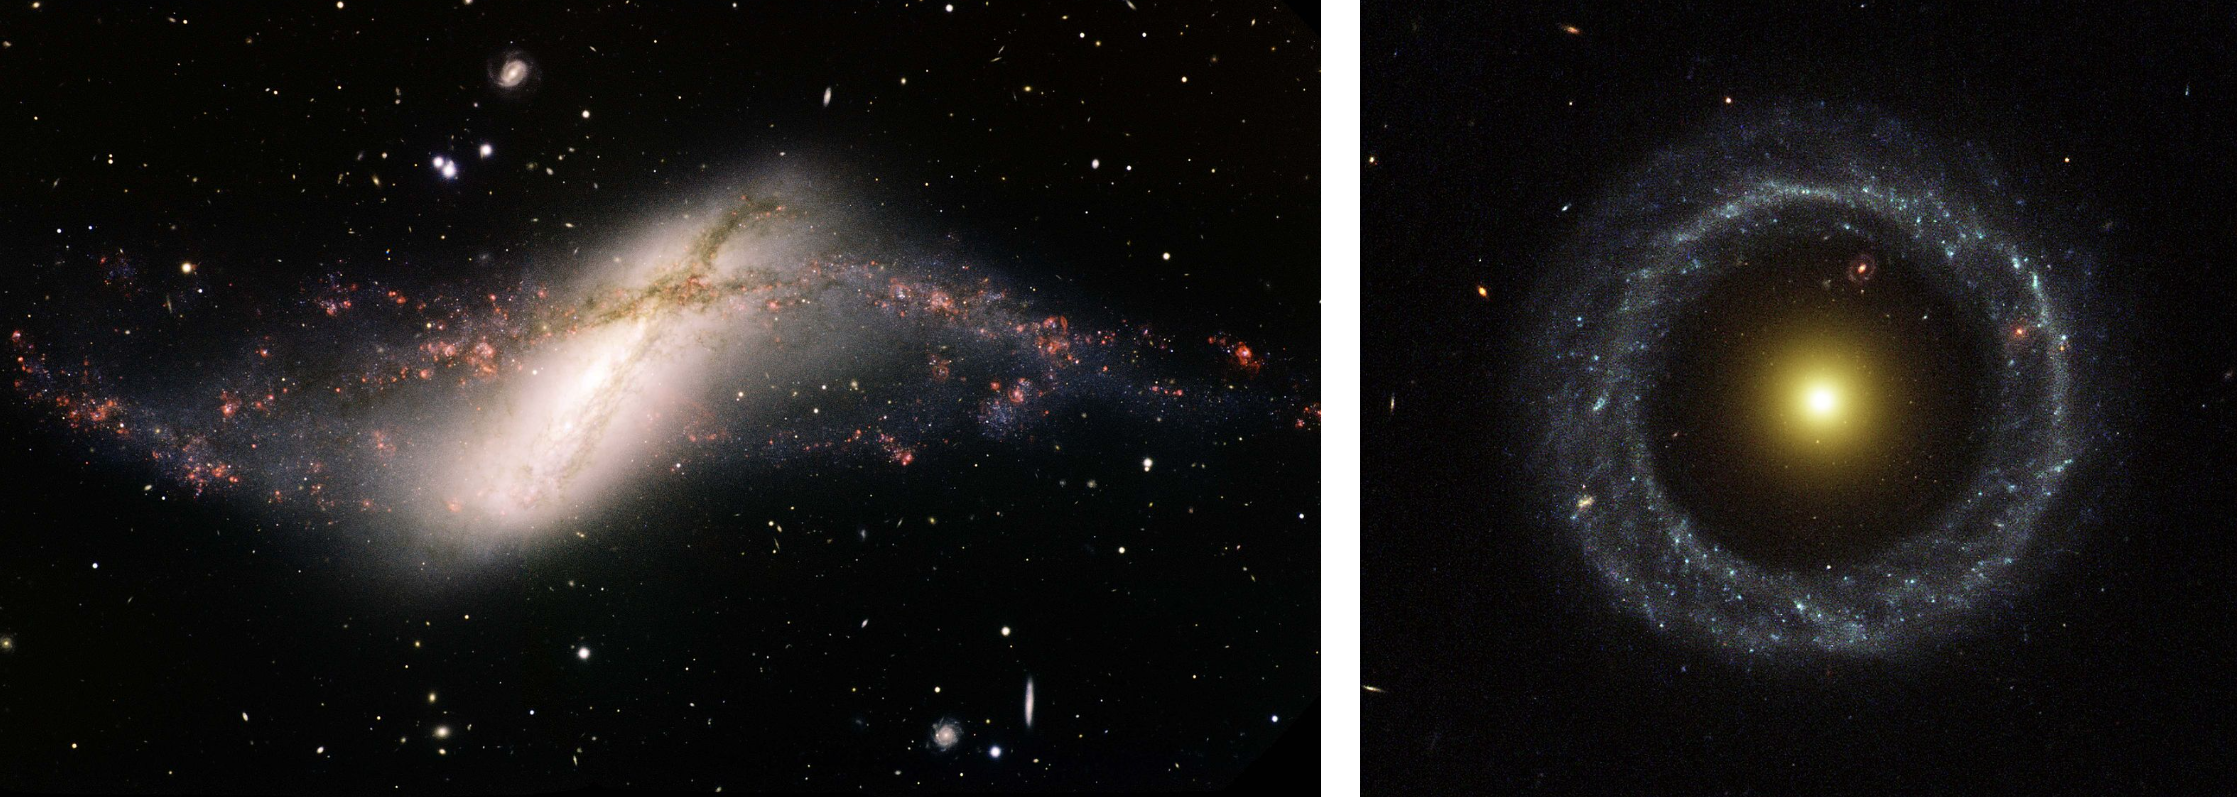
\includegraphics[width=0.8\textwidth]{Imagens/polarehoag.png} 
  \caption[Galáxia de anel polar NGC 660 e galáxia de anel Hoag ]{Galáxia NGC 660 de anel polar, créditos: Gemini Observatory/AURA. Galáxia PGC 54559 de anel Hoag, créditos: NASA, The Hubble Heritage Team (STScI/AURA) e Ray A. Lucas (STScI/AURA).}
  \label{fig:polarehoag} 
\end{figure}

Em 2011, \citeonline{2011MNRAS.418.1834F} fizeram observações para obter a cinemática dos anéis da galáxia PGC 54559 (Hoag's Object) e propuseram que o núcleo e o anel tivessem se formado separadamente. Primeiro, analisaram como o núcleo teria se formado, sendo uma espécie de fóssil ou remanescente de um aglomerado de galáxias que foram se aproximando e eventualmente se fundiram em um elíptico objeto. Também sugeriram que esta pequena galáxia poderia se formar a partir da dissipação ou colapso das estrelas nessa estrutura esférica, por ser pequena em relação às galáxias elípticas que se observa. Quanto ao anel, propuseram que tenha se originado em torno do núcleo esférico a partir de um acréscimo muito lento do meio intergaláctico, proveniente do gás de galáxias que existiam antes de se fundirem. Dessa forma, esse gás poderia lentamente se juntar em torno da região central elíptica, formando um anel, e iniciar o processo de formação de estrelas. Este estudo deixa algumas perguntas como: Por que formaria um anel circular? Por que não formaria um disco como se observa em outros casos (como Messier 81)? Em 2018, Elena Bannikova estudou detalhadamente o potencial e os movimentos de partículas de teste para PGC 54559, observando como realmente seriam as órbitas em torno da estrutura circular anelada. Analisou como a força entre o núcleo esférico e o anel equilibram as forças gravitacionais e descobre que está em uma região que denomina de OSCO\footnote{Denomina-se órbita circular estável mais interna (ISCO), onde o raio ISCO é 3Rg, (Rg = 2GM/c² é o raio de Schwarzschild). Neste caso, as órbitas estáveis estão dentro da última órbita circular estável. Por analogia, órbita circular estável mais externa (OSCO - do inglês \emph{outermost stable circular orbit}).}, Figura~\ref{fig:osco}. Este estudo mostra como o anel circular de Hoag's Object se mantém em equilíbrio e bem definido em torno da região central elíptica da galáxia.

\begin{figure}[h]
  \centering 
  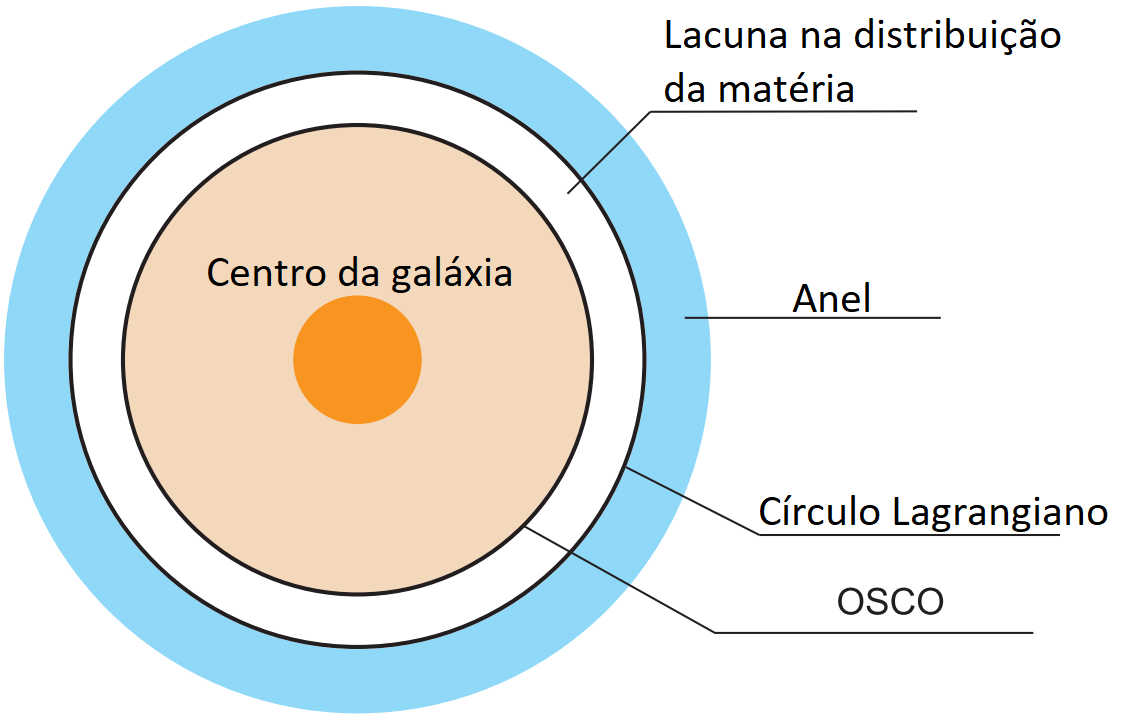
\includegraphics[width=0.65\textwidth]{Imagens/innerring.PNG} 
  \caption[Estabilidade das órbitas em sistemas de anéis do tipo Hoag.]{A estabilidade das órbitas em sistemas de anéis do tipo Hoag. Adaptado de \cite{2018MNRAS.476.3269B}.}
  \label{fig:osco} 
\end{figure}

Recentemente, \citeonline{2024MNRAS.527.4112S} realizaram simulações cosmológicas TNG50\footnote{Simulações cosmológicas que acompanham a formação e evolução das galáxias em um universo de matéria escura fria (CDM, do inglês Cold Dark Matter).} para traçar a origem de estruturas polares em galáxias de anéis polares, descobrindo que estas estruturas são o resultado da estreita interação entre a galáxia hospedeira e sua companheira e que podem aumentar a atividade nuclear da galáxia central e/ou desligar completamente o núcleo ativo. As imagens sintéticas e a distribuição de massa bariônica (Figura~\ref{fig:2024prg}) foram usadas para identificar seis galáxias com anéis polares estelares na simulação, confirmando sua semelhança com as galáxias observadas. Investigaram dois caminhos de formação dos anéis polares estelares: formação de estrelas no gás agregado e interrupção das marés do componente estelar do satélite, observando um aumento constante na inclinação dos anéis ao longo de bilhões de anos. As características das galáxias de anéis polares simuladas, como luminosidades integrais, cores e tamanhos, foram em geral, de acordo com as atuais observações.

\begin{figure}[h]
  \centering 
  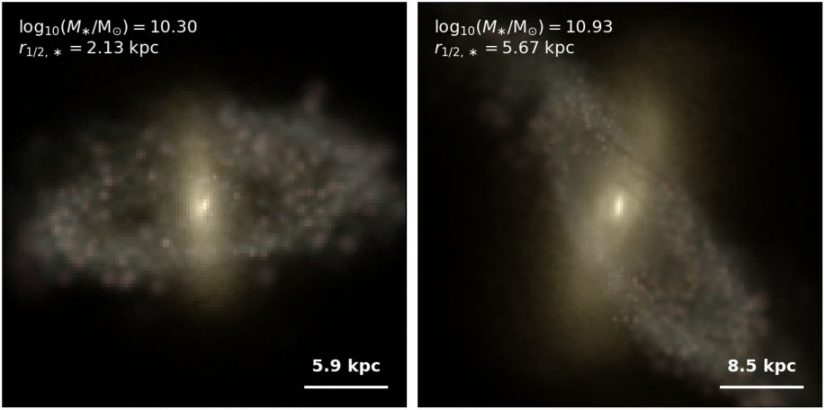
\includegraphics[width=0.8\textwidth]{Imagens/2024prg.PNG} 
  \caption[Simulações cosmológicas de galáxias com anéis polares.]{Imagens de candidatas a galáxias com anéis polares do Illustris TNG50, no canto inferior direito indica a escala das imagens, e no canto superior esquerdo, a massa estelar total e o raio de meia-massa estelar de cada galáxia.}
  \label{fig:2024prg} 
\end{figure}

\citeonline{1974free} apresentaram um modelo para ilustrar a formação dos anéis, por meio de encontros com nuvens de HI (hidrogênio neutro) intergalácticas e as implicações para as propriedades e remanescentes dessas interações. O estudo apresenta modelos específicos de galáxias peculiares com base no conceito proposto de encontros galáxia-nuvem, em que a existência dessas nuvens moderadamente densas é postulada com base em evidências de observações de nuvens HI em vários sistemas galácticos, demonstrando que a morfologia depende da galáxia original, estágio evolutivo, ângulo de incidência e velocidade dos corpos no evento. Algumas observações de RGs, como a Cartwheel e o anel Lindsay-Shapley, encontraram evidências das galáxias responsáveis pela colisão dentro da faixa de distância, velocidades e ângulos de posição, esperados para interações colisionais frontais \cite{2009madore} como ilustra a Figura~\ref{fig:g3}.

\begin{figure}[h]
  \centering 
  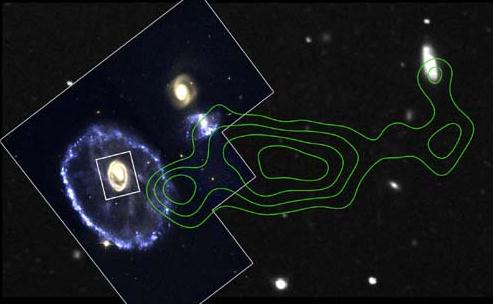
\includegraphics[width=0.8\textwidth]{Imagens/cartwheel2_hst.jpg} 
  \caption[Galáxia Cartwheel e sua interagente.]{A grande galáxia do grupo Cartwheel sobreviveu a uma colisão com uma pequena galáxia viajante, o que fez possível a formação de um anel expansivo ao redor do núcleo galáctico com várias estrelas se formando. Nesta imagem observa-se o rastro, em verde, do gás e poeira em ondas de rádio, mapeando a distribuição de hidrogênio neutro e identificando a galáxia na extrema direita a cerca de 250 mil anos-luz, responsável pelo evento. Créditos: J.Higdon (NRAO), C.Struck, P.Appleton (ISU), K.Borne (Hughes STX), R.Lucas (STScI), NASA.}
  \label{fig:g3} 
\end{figure}

\section{Observação de propriedades}

Nos últimos anos, houve grande avanço no estudo em múltiplas bandas em RGs, para analisar propriedades dos anéis, como a taxa de formação estelar e gradiente de cor radial. Em 2008, \citeonline{2008ASPC..381..128A} apresentaram resultados de um levantamento GALEX e SPITZER com RGs colisionais, com combinação de imagens e espectroscopia UV e infravermelho médio, investigando a relação entre as regiões de formação estelares massivas e o aquecimento da poeira nos anéis. Em Cartwheel, por exemplo, analisaram o desenvolvimento do anel e suas doze fontes luminosas ULXs (ultraluminosas fontes de raio-X), revelando um gigantesco disco UV externo. Em 2012, \citeonline{prestwich2012} descobriram uma correlação entre o número dessas fontes luminosas através de simulações da população binária da NGC 922 e Cartwheel, usando o código StarTrack para entender a formação de ULXs. Tanto NGC 922 quanto Cartwheel são PRGs com anel expansivo e de formação estelar. A população ULXs em ambos os objetos foi analisada e comparada, levando em consideração fatores como metalicidade e taxa de formação de estrelas, sugerindo que possam ser dominadas por sistemas com forte acreção de vento por buracos negros supergigantes de colapso-direto, contribuição importante para o seu papel na evolução das galáxias. 

\begin{figure}[h]
  \centering 
  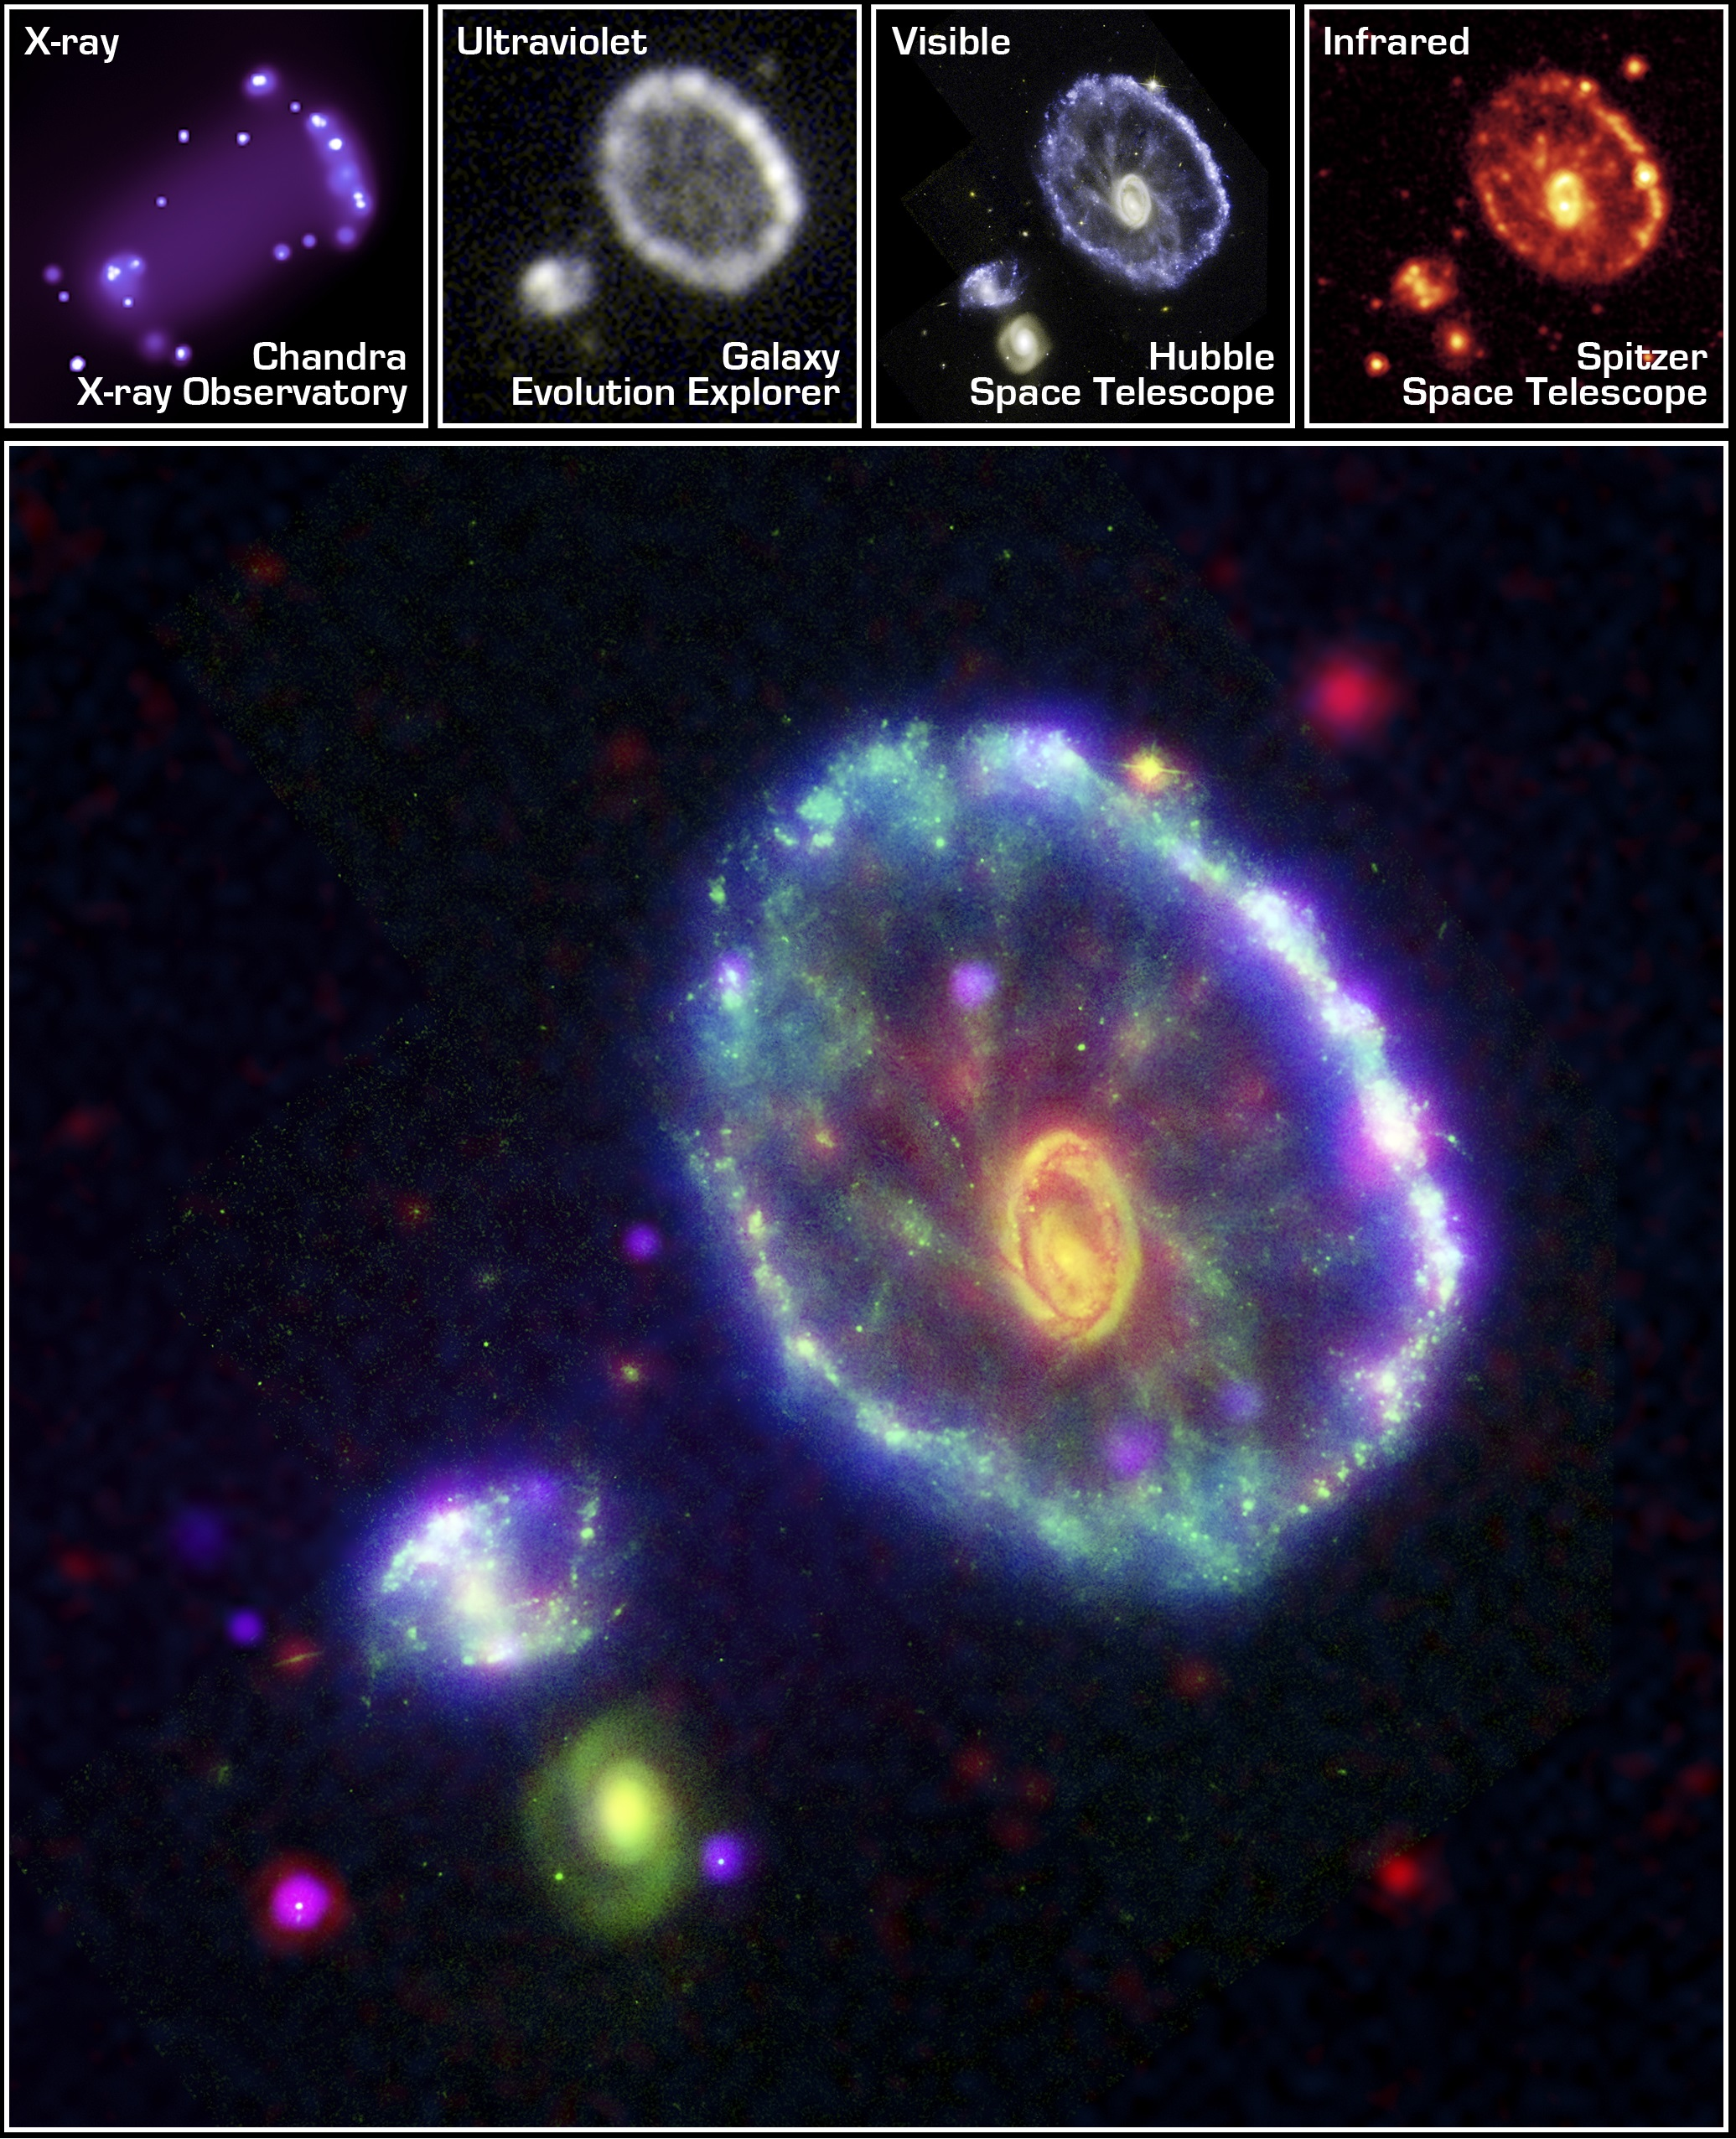
\includegraphics[width=0.65\textwidth]{Imagens/Cartwheel04.jpg} 
  \caption[Composição de imagens de Cartwheel.]{Combinação de dados de quatro observatórios: Observatório de Raios-X Chandra (roxo); satélite Galaxy Evolution Explorer (ultravioleta/azul); Telescópio Espacial Hubble (visível/verde); Telescópio Espacial Spitzer (infravermelho/vermelho). Créditos: composição: NASA/JPL/Caltech/P.Appleton et al.; raio-X: NASA/CXC/A.Wolter \& G.Trinchieri et al.}
  \label{fig:cart4} 
\end{figure}

Quando estrelas massivas explodem como supernovas, deixam para trás estrelas de nêutrons e buracos negros, que podem possuir estrelas próximas e se tornarem poderosas fontes de raios-X muito brilhantes ao retirar matéria de suas companheiras. Por possuírem essas fontes ULXs espalhadas pelo anel, estas galáxias se tornam interessantes laboratórios para sondar os objetos mais pesados do universo, os buracos negros, e conforme \citeonline{2010MNRAS.406.1116P} sugeriram, a mais brilhante fonte desses raios-X, seria provavelmente, um buraco negro de massa intermediária.


 ... a complementar ...



ler
Houve três grandes tentativas de explicar a origem das galáxias aneladas (Freeman e de Vaucouleurs 1974; Theys e Spiegel 1976; Lynds e Toomre 1976). Todas essas abordagens envolvem a colisão de uma nuvem ou galáxia com outra galáxia de uma maneira especial, geralmente através do centro da galáxia, que se torna a galáxia anelada. A perturbação resultante, quase simétrica, é proposta para explicar a formação do anel. Naturalmente, a presença de companheiros próximos é de grande importância para esses tipos de teorias, e os exemplos atuais de galáxias aneladas com companheiros fornecem muitos casos onde redshifts, magnitudes e espectros podem ser obtidos para verificar essas teorias. Por outro lado, será muito interessante descobrir exemplos onde não há companheiros aparentes nas proximidades do anel. \cite{1987arpmadore}
